% header copied from final project 
% Preamble:

%Here's where packages go. 

\documentclass{article} %lots of other options here, like amsart, among others
\usepackage{amsmath} %includes lots of mathematical symbols and content
\usepackage{lipsum} % For blind text
\usepackage{fullpage}
\usepackage{imakeidx} %make index
\usepackage{float}
\makeindex[title=Index of Terms, columns=3, columnsep=20pt, intoc]

\usepackage{enumerate}
\usepackage{array,tabularx,multirow} %Helpful for certain tables and table features
\usepackage{graphicx}
\graphicspath{ {./Images/} }
\usepackage{mermaid}
\usepackage{wrapfig}
% \usepackage{animate} % this is for the newly learned animated package
\usepackage{xcolor} % Required for color names
\definecolor{linkblue}{HTML}{56B7E6}
\usepackage{hyperref}%%Generally hyperref should be the last package loaded.
\usepackage{pgfplots}
\pgfplotsset{compat=1.18}

\usepackage{tikz}
\usetikzlibrary{calc,patterns,angles,quotes,graphs,graphs.standard,arrows.meta,positioning,fit} % useful set of TikZ libraries for various diagram elements

\hypersetup{
    colorlinks=true,
    linkcolor=linkblue,   % TOC entries, TOC/index page numbers, internal refs
    urlcolor=linkblue,    % external URLs
    citecolor=linkblue,
    linktoc=page          % make page nums clicable
}

\definecolor{rcrcrf}{rgb}{0.10980392156862745,0.10980392156862745,0.12156862745098039}
\definecolor{ududff}{rgb}{0.30196078431372547,0.30196078431372547,1}
\definecolor{xdxdff}{rgb}{0.49019607843137253,0.49019607843137253,1}
\definecolor{wewdxt}{rgb}{0.43137254901960786,0.42745098039215684,0.45098039215686275}

% italicize new terms, and add them to the index
\newcommand{\newterm}[1]{\textit{#1}\index{#1}}

% TOC edits - nonstandard
\usepackage{tocloft}
\renewcommand{\contentsname}{Table of Contents} % Change title text
\renewcommand{\cfttoctitlefont}{\hfill\Large\bfseries} % Center and style title
\renewcommand{\cftaftertoctitle}{\hfill} % Required for centering
\renewcommand{\cftsecfont}{\bfseries} % Section titles bold
\renewcommand{\cftsecpagefont}{\bfseries} % Section page numbers bold
\renewcommand{\cftsubsecfont}{\itshape\/} % Subsection titles italic

% Begin Cover Page
\title{Week 10 — TikZ Diagrams}
\author{Arjan Singh Ellingson}
%\date{August 24th, 2026}
\date{\today}

\begin{document}
% Your submission should include:

% Two sufficiently different hand-coded TikZ figures that include various style elements (colors, line thicknesses, dashing, etc.) 
% Three different sets of TikZ figures made via GeoGebra. Use a variety of elements like styles, locations, shapes, etc. 
% Optional: Clean up the TikZ code generated via GeoGebra  
% Optional: Have your favorite AI program generate the TikZ figures for you and compare it to what you had GeoGebra do. Reflect on how well this process worked. 

\section{Handcoded TikZ Figures}
This is a figure from a previous chapter I wrote for my educational curriculum job to describe a circular motion of a billiard ball bound to a string.

\begin{figure}[H]
    \begin{center}
        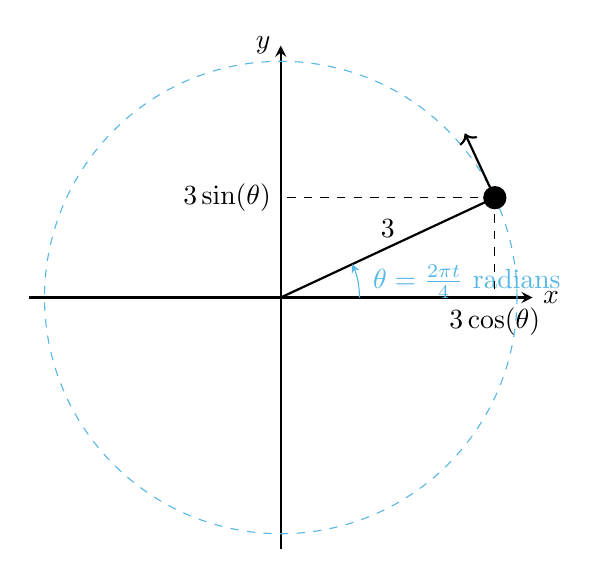
\begin{tikzpicture}[declare function={angle=25;},bullet/.style={inner
                        sep=1pt,fill,draw,circle,solid}, scale=1] % right-sized to match other circle diagrams in this chapter
            % Axis
            \draw[thick,-stealth,black] (-3.2,0)--(3.2,0) node[right] {$x$}; % x axis
            \draw[thick,-stealth,black] (0,-3.2)--(0,3.2) node[left] {$y$}; % y axis
            % Rest
            \draw [dashed, linkblue] (0,0) circle (3);
            \draw[thick] (0,0) -- (angle:3.0) node [midway, above] {3};
            \draw[linkblue] (1.05, 0.2) node[right] {$\theta = \frac{2\pi t}{4}\text{ radians}$};
            \draw[-stealth,linkblue] (1,0) arc (0:angle:1);
            \draw[dashed, black] (2.71892336110995, 1.267854785222098) -- (2.71892336110995, 0)
            node[below] {$3 \cos(\theta)$}; % vertical
            \draw[dashed, black] (2.71892336110995, 1.267854785222098) -- (0, 1.267854785222098)
            node[left] {$3 \sin(\theta)$}; % horizontal
            \filldraw[black] (angle:3.0) circle(4pt);
            \draw[->, thick] (2.71892336110995, 1.267854785222098) --
            (2.71892336110995 - 3 * 0.1267, 1.267854785222098 + 3 * 0.2718);
        \end{tikzpicture}
    \end{center}
    \caption{A diagram of our ball and string scenario.}
    \label{fig:billiardBall}
\end{figure}

This is a diagram I drew a while back for describing the FBD of a box on an inclined plane.
\begin{figure}[H]
    \centering
    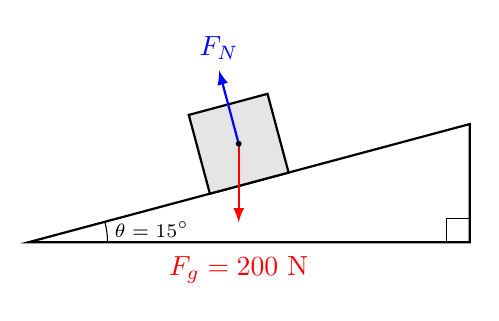
\begin{tikzpicture}
        \draw[thick, black] (0,0) -- (5.6, 0) -- (5.6, 1.5) -- cycle;
        \draw[] (5.3, 0) -- (5.3, 0.3) -- (5.6, 0.3);
        \draw[] (1, 0) arc (0:15:1) node[right, font = \scriptsize, yshift = -0.1cm]
            {$\theta = 15^{\circ}$};
        \draw[thick, black, fill=gray!20] (2.3, 0.616) -- (3.3, 0.884) --
        (3.032, 1.884) -- (2.032, 1.616) -- cycle;
        \draw[-latex, thick, blue] (2.666, 1.25) -- (2.416, 2.183)
        node[above] {$F_N$};
        \draw[-latex, thick, red] (2.666, 1.25) -- (2.666, 0.25)
        node[below, yshift = -0.3cm] {$F_g = 200\text{ N}$};
        \draw[black, fill=black] (2.666, 1.25) circle (0.03cm);
    \end{tikzpicture}
    \caption{A box sits on a $15^\circ$ inclined plane. A gravitational force of $200\text{ N}$ acts downward while a normal force acts perpendicular to the surface. The ultimate goal of this problem is to figure out the net force acting on the box along the incline.}
    \label{fig:fbd}
\end{figure}

\section{Geogebra generated ones}
I moved the library and color def stuff up to the preamble for better organization.


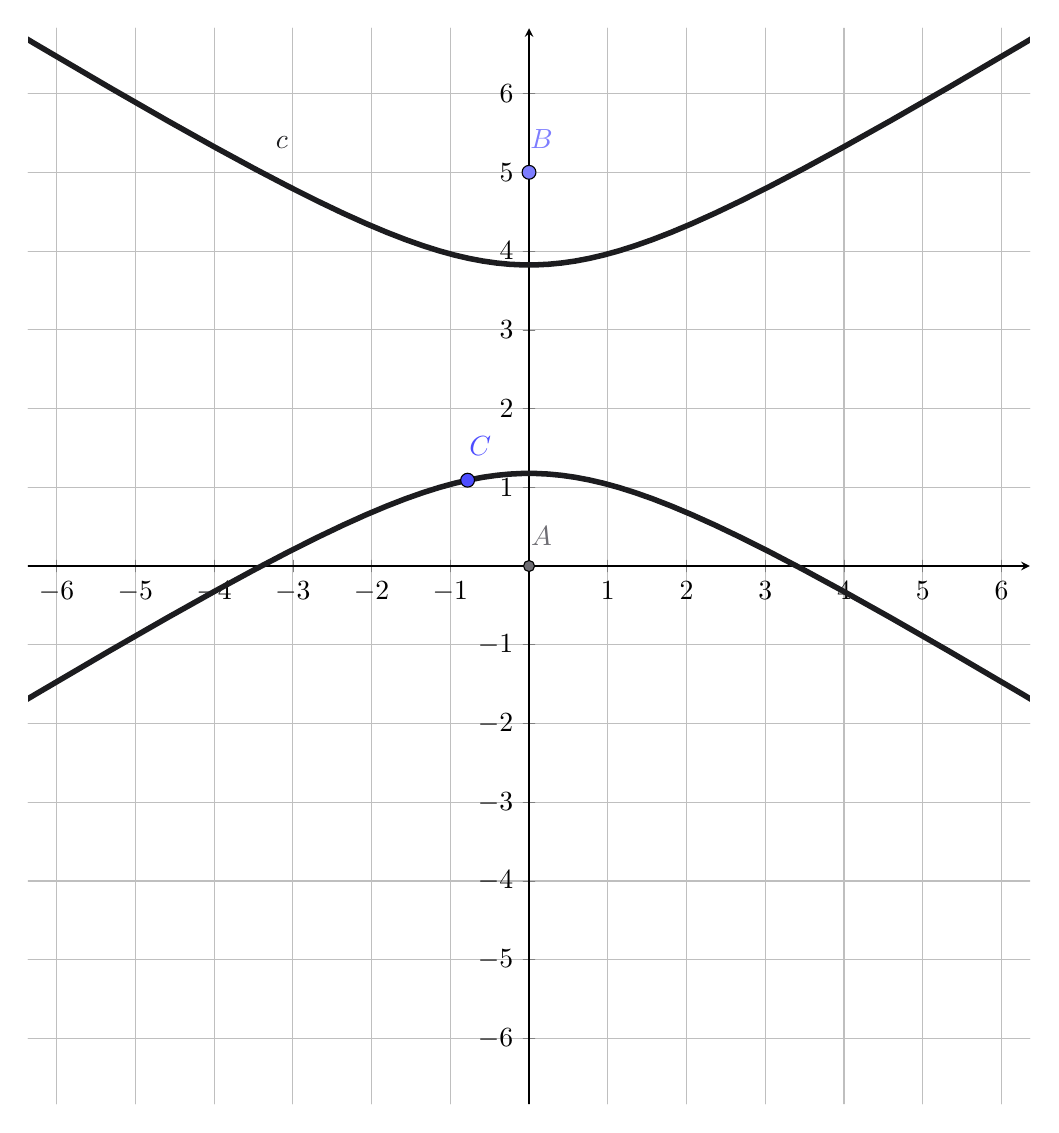
\begin{tikzpicture}[line cap=round,line join=round,>=Stealth,x=1cm,y=1cm]
    \begin{axis}[
            x=1cm,y=1cm,
            axis lines=middle,
            ymajorgrids=true,
            xmajorgrids=true,
            xmin=-6.36,
            xmax=6.36,
            ymin=-6.83,
            ymax=6.83,
            xtick={-6,-5,...,6},
            ytick={-6,-5,...,6},]
        \clip(-6.36,-6.83) rectangle (6.36,6.83);
        \draw [samples=50,domain=-0.95:0.95,rotate around={90:(0,2.5)},xshift=0cm,yshift=2.5cm,line width=2pt,color=rcrcrf] plot ({1.3233528654327626*(1+(\x)^2)/(1-(\x)^2)},{2.121022676340566*2*(\x)/(1-(\x)^2)});
        \draw [samples=50,domain=-0.95:0.95,rotate around={90:(0,2.5)},xshift=0cm,yshift=2.5cm,line width=2pt,color=rcrcrf] plot ({1.3233528654327626*(-1-(\x)^2)/(1-(\x)^2)},{2.121022676340566*(-2)*(\x)/(1-(\x)^2)});
        \begin{scriptsize}
            \draw [fill=wewdxt] (0,0) circle (2pt);
            \draw[color=wewdxt] (0.16,0.38) node {$A$};
            \draw [fill=xdxdff] (0,5) circle (2.5pt);
            \draw[color=xdxdff] (0.16,5.42) node {$B$};
            \draw [fill=ududff] (-0.78,1.09) circle (2.5pt);
            \draw[color=ududff] (-0.62,1.52) node {$C$};
            \draw[color=rcrcrf] (-3.14,5.38) node {$c$};
        \end{scriptsize}
    \end{axis}
\end{tikzpicture}


\definecolor{xdxdff}{rgb}{0.49019607843137253,0.49019607843137253,1}
\definecolor{ududff}{rgb}{0.30196078431372547,0.30196078431372547,1}
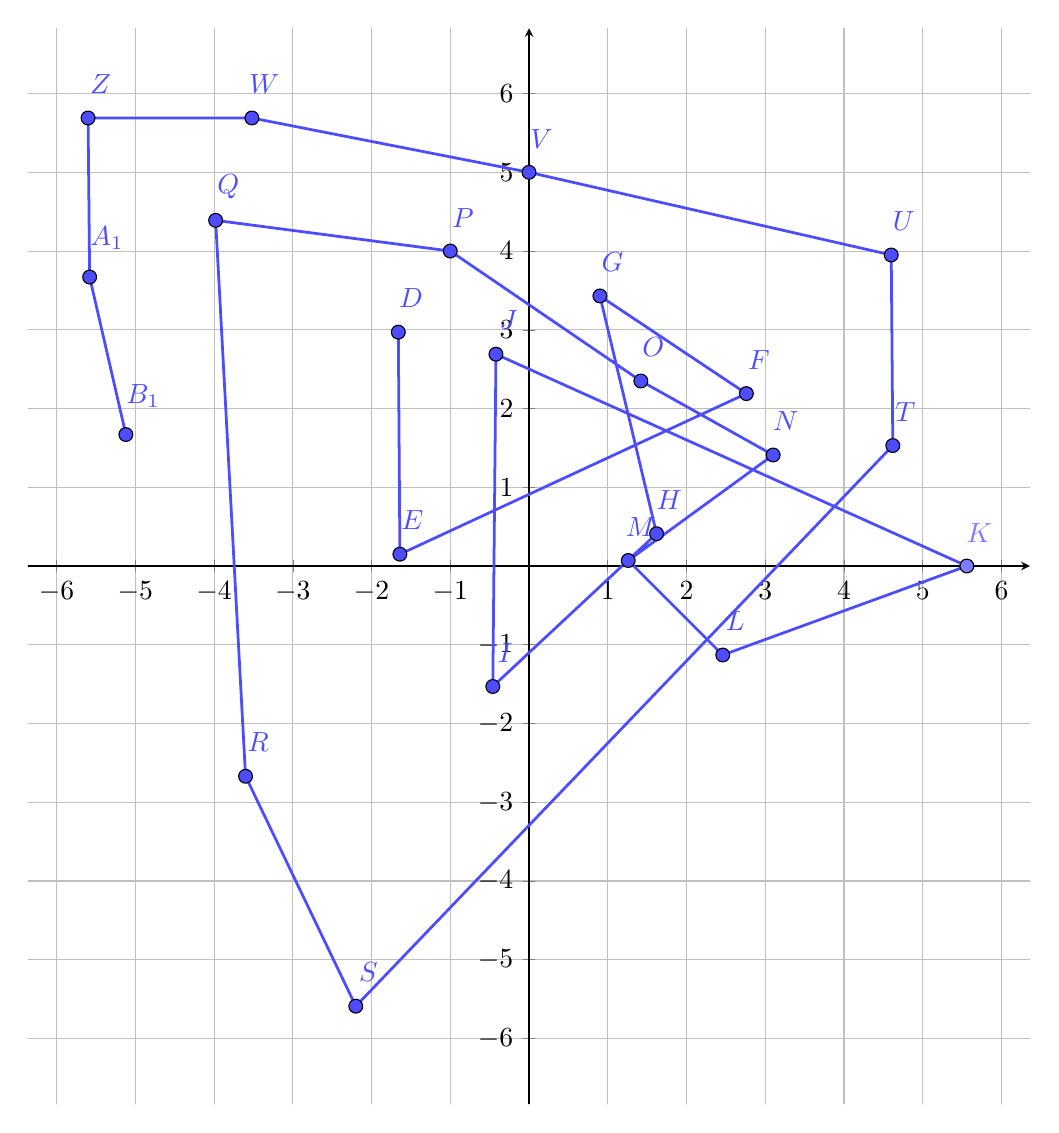
\begin{tikzpicture}[line cap=round,line join=round,>=Stealth,x=1cm,y=1cm]
    \begin{axis}[
            x=1cm,y=1cm,
            axis lines=middle,
            ymajorgrids=true,
            xmajorgrids=true,
            xmin=-6.36,
            xmax=6.36,
            ymin=-6.83,
            ymax=6.83,
            xtick={-6,-5,...,6},
            ytick={-6,-5,...,6},]
        \clip(-6.36,-6.83) rectangle (6.36,6.83);
        % connect the points in alphabetical order: D, E, ..., W, Z, A_1, B_1
        \draw [color=ududff,line width=1pt]
        (-1.66,2.97) -- (-1.64,0.15) -- (2.76,2.19) -- (0.9,3.43) -- (1.62,0.41) --
        (-0.46,-1.53) -- (-0.42,2.69) -- (5.56,0) -- (2.46,-1.13) -- (1.26,0.07) --
        (3.1,1.41) -- (1.42,2.35) -- (-1,4) -- (-3.98,4.39) -- (-3.6,-2.67) --
        (-2.2,-5.59) -- (4.62,1.53) -- (4.6,3.95) -- (0,5) -- (-3.52,5.69) --
        (-5.6,5.69) -- (-5.58,3.67) -- (-5.12,1.67);
        \begin{scriptsize}
            \draw [fill=ududff] (-1.66,2.97) circle (2.5pt);
            \draw[color=ududff] (-1.5,3.4) node {$D$};
            \draw [fill=ududff] (-1.64,0.15) circle (2.5pt);
            \draw[color=ududff] (-1.48,0.58) node {$E$};
            \draw [fill=ududff] (2.76,2.19) circle (2.5pt);
            \draw[color=ududff] (2.92,2.62) node {$F$};
            \draw [fill=ududff] (0.9,3.43) circle (2.5pt);
            \draw[color=ududff] (1.06,3.86) node {$G$};
            \draw [fill=ududff] (1.62,0.41) circle (2.5pt);
            \draw[color=ududff] (1.78,0.84) node {$H$};
            \draw [fill=ududff] (-0.46,-1.53) circle (2.5pt);
            \draw[color=ududff] (-0.3,-1.1) node {$I$};
            \draw [fill=ududff] (-0.42,2.69) circle (2.5pt);
            \draw[color=ududff] (-0.26,3.12) node {$J$};
            \draw [fill=xdxdff] (5.56,0) circle (2.5pt);
            \draw[color=xdxdff] (5.72,0.42) node {$K$};
            \draw [fill=ududff] (2.46,-1.13) circle (2.5pt);
            \draw[color=ududff] (2.62,-0.7) node {$L$};
            \draw [fill=ududff] (1.26,0.07) circle (2.5pt);
            \draw[color=ududff] (1.42,0.5) node {$M$};
            \draw [fill=ududff] (3.1,1.41) circle (2.5pt);
            \draw[color=ududff] (3.26,1.84) node {$N$};
            \draw [fill=ududff] (1.42,2.35) circle (2.5pt);
            \draw[color=ududff] (1.58,2.78) node {$O$};
            \draw [fill=ududff] (-1,4) circle (2.5pt);
            \draw[color=ududff] (-0.84,4.42) node {$P$};
            \draw [fill=ududff] (-3.98,4.39) circle (2.5pt);
            \draw[color=ududff] (-3.82,4.82) node {$Q$};
            \draw [fill=ududff] (-3.6,-2.67) circle (2.5pt);
            \draw[color=ududff] (-3.44,-2.24) node {$R$};
            \draw [fill=ududff] (-2.2,-5.59) circle (2.5pt);
            \draw[color=ududff] (-2.04,-5.16) node {$S$};
            \draw [fill=ududff] (4.62,1.53) circle (2.5pt);
            \draw[color=ududff] (4.78,1.96) node {$T$};
            \draw [fill=ududff] (4.6,3.95) circle (2.5pt);
            \draw[color=ududff] (4.76,4.38) node {$U$};
            \draw [fill=ududff] (0,5) circle (2.5pt);
            \draw[color=ududff] (0.16,5.42) node {$V$};
            \draw [fill=ududff] (-3.52,5.69) circle (2.5pt);
            \draw[color=ududff] (-3.36,6.12) node {$W$};
            \draw [fill=ududff] (-5.6,5.69) circle (2.5pt);
            \draw[color=ududff] (-5.44,6.12) node {$Z$};
            \draw [fill=ududff] (-5.58,3.67) circle (2.5pt);
            \draw[color=ududff] (-5.36,4.16) node {$A_1$};
            \draw [fill=ududff] (-5.12,1.67) circle (2.5pt);
            \draw[color=ududff] (-4.9,2.16) node {$B_1$};
        \end{scriptsize}
    \end{axis}
\end{tikzpicture}

This is a figure with a 12-sided polygon, semi circle, and conic.

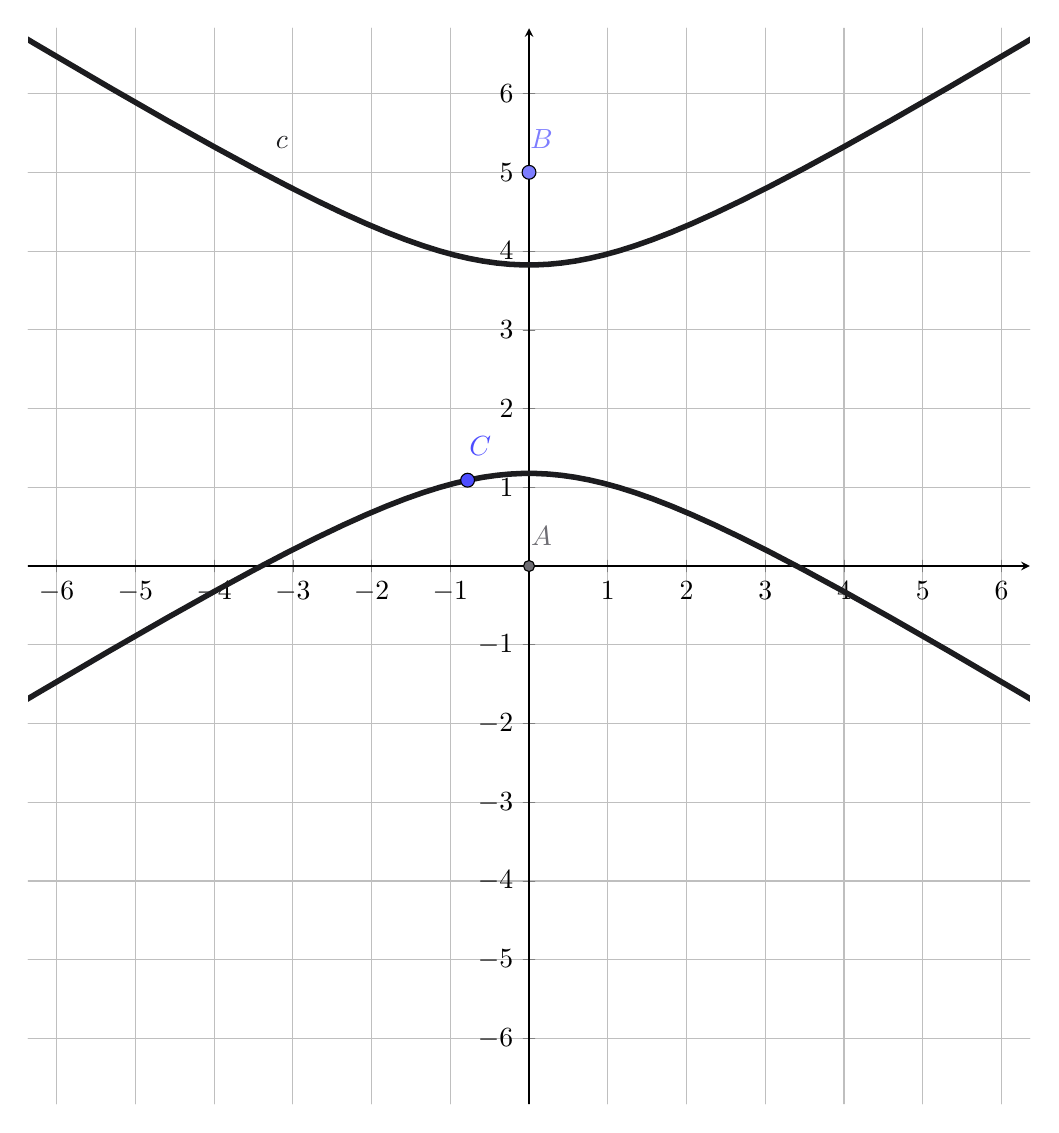
\begin{tikzpicture}[line cap=round,line join=round,>=Stealth,x=1cm,y=1cm]
    \begin{axis}[
            x=1cm,y=1cm,
            axis lines=middle,
            ymajorgrids=true,
            xmajorgrids=true,
            xmin=-6.36,
            xmax=6.36,
            ymin=-6.83,
            ymax=6.83,
            xtick={-6,-5,...,6},
            ytick={-6,-5,...,6},]
        \clip(-6.36,-6.83) rectangle (6.36,6.83);
        \draw [samples=50,domain=-0.95:0.95,rotate around={90:(0,2.5)},xshift=0cm,yshift=2.5cm,line width=2pt,color=rcrcrf] plot ({1.3233528654327626*(1+(\x)^2)/(1-(\x)^2)},{2.121022676340566*2*(\x)/(1-(\x)^2)});
        \draw [samples=50,domain=-0.95:0.95,rotate around={90:(0,2.5)},xshift=0cm,yshift=2.5cm,line width=2pt,color=rcrcrf] plot ({1.3233528654327626*(-1-(\x)^2)/(1-(\x)^2)},{2.121022676340566*(-2)*(\x)/(1-(\x)^2)});
        \begin{scriptsize}
            \draw [fill=wewdxt] (0,0) circle (2pt);
            \draw[color=wewdxt] (0.16,0.38) node {$A$};
            \draw [fill=xdxdff] (0,5) circle (2.5pt);
            \draw[color=xdxdff] (0.16,5.42) node {$B$};
            \draw [fill=ududff] (-0.78,1.09) circle (2.5pt);
            \draw[color=ududff] (-0.62,1.52) node {$C$};
            \draw[color=rcrcrf] (-3.14,5.38) node {$c$};
        \end{scriptsize}
    \end{axis}
\end{tikzpicture}
Future improvements could include shrinking the grid sizes, adding labels to all points and curves, improving the color scheme for better visibility, and possibly adding interactive elements for dynamic visualization.
\end{document}